\chapter{Feature Extraction}
\label{ch:feature-extraction}

As an acoustic wave propagated through space over time, the speech signal is not appropriate to be evaluated by an ASR system. In order to deliver decent outcomes, a good parametric representation must be provided. This task is performed by the \textbf{feature extraction process}, which transforms a speech signal into a sequence of characterized measurements, i.e. features. The selected representation compress the speech data by eliminating information not pertinent to the phonetic analysis and enhancing those aspects of the signal that contribute significantly to the detection of phonetic differences, \refbib{Davis \& Mermelstein}{davis.mermelstein.1980}. According to \refbib{Wolf}{wolf.1972}, the ideal features should:

\begin{itemize}\itemsep0pt
    \item occur naturally and frequently in normal speech;
    \item be easily measurable;
    \item vary highly among speakers and be very consistent for each speaker;
    \item not change over time nor be affected by the speaker's health;
    \item be robust to reasonable background noise and to transmission
    characteristics;
    \item be difficult to be artificially produced;
    \item not be easily modifiable by the speaker.
\end{itemize}

Features may be categorized based on vocal tract or behavioral aspects, divided in (1) short-time spectral, (2) spectro-temporal, (3) prosodic and (4) high level, \refbib{Pinheiro}{pinheiro.2013}. Short-time spectral features are usually calculated using millisecond length windows and describe the voice spectral envelope, composed of supralaryngeal properties of the vocal tract (e.g. timbre). Spectro-temporal and prosodic occur over time (e.g., rhythm and intonation), and high level features occur during the conversation (e.g., accent).

The parametric representations evaluated in \refbib{Davis \& Mermelstein}{davis.mermelstein.1980} may be divided into those based on the Fourier spectrum, such as Mel-Frequency Cepstrum Coefficients (MFCC) and Linear Frequency Cepstrum Coefficients (LFCC), and those based on the Linear Prediction Spectrum, such as Linear Prediction Coefficients (LPC), Reflection Coefficients (RC) and Linear Prediction Cepstrum Coefficients (LPCC). The better evaluated representation was the MFCC, with minimum and maximum accuracy of 90.2\% and 99.4\%, respectively, leading to its choice as the parametric representation in this work.

\section{Mel-Frequency Cepstral Coefficient}

MFCC is a highly used parametric representation in the area of voice processing, due to its similarity with the way the human ear operates. Despite the fact the ear is divided in three sections, i.e., outer, middle and inner ears, only the last is mimicked. The mechanical pressure waves produced by the triad hammer-anvil-stirrup are received by the \textbf{cochlea} (\figureref{cochlea}), a spiral-shaped cavity with a set of inner hair cells attached to a membrane (the basilar membrane) and filled with a liquid. This structure converts motion to neural activity through a non-uniform spectral analysis, \refbib{Rabiner \& Schafer}{rabiner.schafer.2007}, and passes it to the pattern recognizer in the brain.

\begin{figure}[ht]
    \centering
    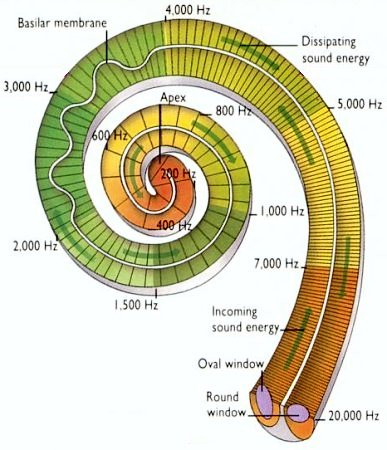
\includegraphics[width=0.5\textwidth]{cochlea}
    \caption{Cochlea divided by frequency regions, \refbib{ScienceBlogs}{scienceblogs.2010.05.10}.}
    \label{fig:cochlea}
\end{figure}

A key factor in the perception of speech and other sounds is \textbf{loudness}, a quality related to the physical property of the sound pressure level. Loudness is quantified by relating the actual sound pressure level of a pure tone (in dB relative to a standard reference level) to the perceived loudness of the same tone (in a unit called phons) over the range of human hearing (20 Hz–20 kHz), \refbib{Rabiner \& Schafer}{rabiner.schafer.2007}. As shown in \figureref{loudness}, a 100 Hz tone at 60 dB is equal in loudness to a 1000 Hz tone at 50 dB, both having the \textbf{loudness level} of 50 phons (by convention).

\begin{figure}[ht]
    \centering
    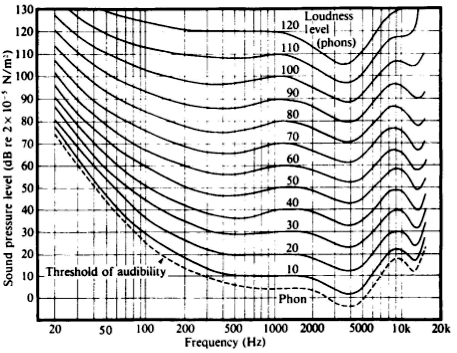
\includegraphics[width=0.6\textwidth]{loudness}
    \caption{Loudness level for human hearing, \refbib{Fletcher \& Munson}{fletcher.munson.1933}.}
    \label{fig:loudness}
\end{figure}

\subsection{The Mel Scale}

The \textbf{mel scale} is the result of an experiment conducted by \refbib{Stevens, Volkmann and Newman}{stevens.volkmann.newman.1937} intended to measure the perception of a pitch and construct a scale based on it. Each observer was asked to listen to two tones, one in the fixed frequencies 125, 200, 300, 400, 700, 1000, 2000, 5000, 8000 and 12000 Hz, and the other free to have its frequency varied by the observer for each fixed frequency of the first tone. An interval of 2 seconds separated both tones. The observers were instructed to say in which frequency the second tone was ``half the loudness" of the first. A geometric mean was taken from the observers' answers and a measure of 1000 mels was assigned to the frequency of 1000 Hz, 500 mels to the frequency sounding half as high (as determined by Fig. 1 in \refbib{Stevens et. al.}{stevens.volkmann.newman.1937}) and so on.

Decades after the scale be defined, \refbib{O'Shaughnessy}{oshaughnessy.1987} presented an equation to convert frequencies in Hertz to frequencies in mels:

\begin{equation}
    f_{mel} = 2595 log_{10}(1 + \frac{f}{700}).
    \label{eq:mel_conversion}
\end{equation}

\noindent Being logarithmic, the growth of a mel-frequency curve is slow when \equationref{mel_conversion} is applied to a linear growth of the frequency in Hertz. Sometimes the mel conversion is used only for frequencies higher than 1000 Hz, while in lower, $f_{mel}$ and $f_{Hz}$ share the same value. In this work all conversions will use \equationref{mel_conversion}, as shown by \figureref{mel_scale}.

\begin{figure}[ht]
    \centering
    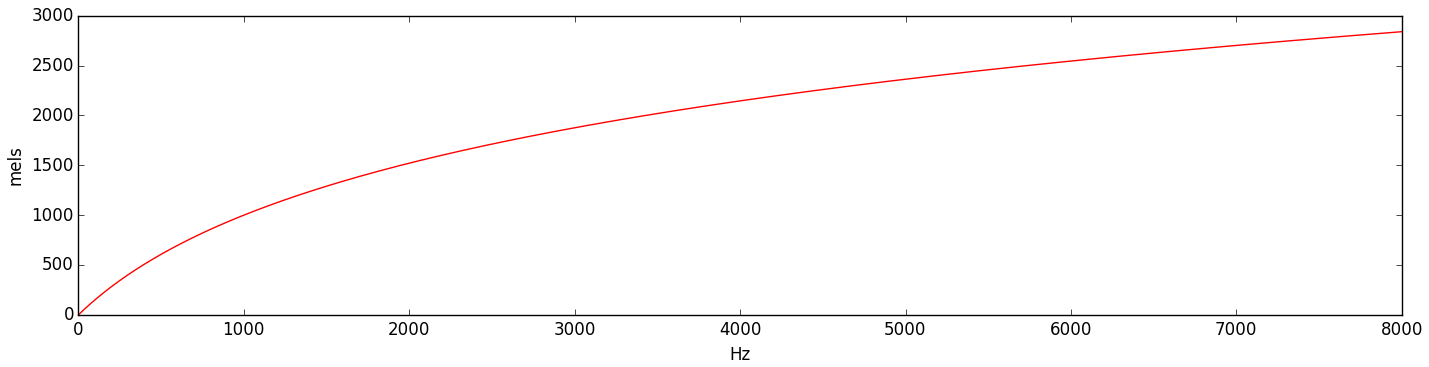
\includegraphics[width=\textwidth]{mel_scale}
    \caption{The logarithm curve of the mel scale.}
    \label{fig:mel_scale}
\end{figure}

\subsection{Extraction Process}

In an ASR system the feature extraction module receives a raw speech signal and returns a vector of cepstral features in mel scale (see \figureref{mfcc-flow}). The number of features in each frame is defined at the moment of extraction (e.g., 6, 13 or 19), but the user has the option to append time variations of the MFCCs (i.e., delta coefficients) in order to improve the representation.

\begin{figure}[ht]
    \centering
    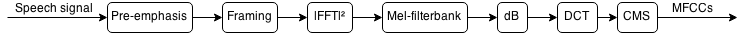
\includegraphics[width=\textwidth]{mfcc-flow}
    \caption{Modular representation of the MFCC extraction.}
    \label{fig:mfcc-flow}
\end{figure}

%Pre-emphasis

As the human voice is concentrated in the lower frequencies (see \figureref{preemphasis}), the higher ones are enhanced to improve the classification. A first order Finite Impulse Response (FIR) filter is used,

\begin{equation}
    s_{emph}[n] = s[n] - a \cdot s[n - 1],
    \label{eq:preemphasis}
\end{equation}

\noindent with values of $a$ usually in the interval $[0.95, 0.98]$, \refbib{Bimbot et. al.}{bimbot.et.al.2004}. This is an optional stage of the MFCC extraction process.

\begin{figure}[ht]
    \centering
    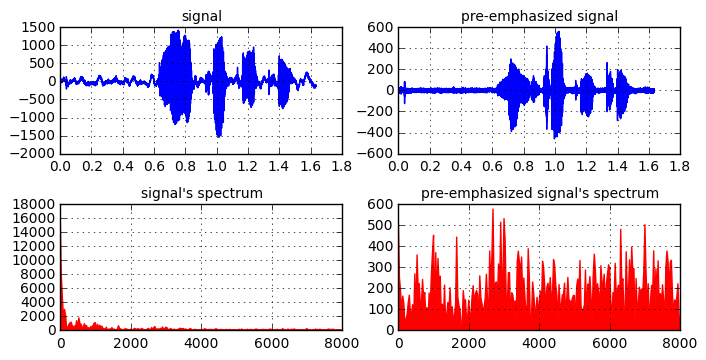
\includegraphics[width=\textwidth]{preemphasis}
    \caption{Raw (left) and pre-emphasized (right) speech signal, with respective spectral magnitudes (at bottom in red).}
    \label{fig:preemphasis}
\end{figure}

%Framing

The first mandatory stage of the feature process is the division of the input signal in overlapping frames, by the application of a sliding window (commonly Hamming, to taper the signal on the ends and reduce the side effects, \refbib{Bimbot et. al.}{bimbot.et.al.2004}). The window has a width in the order of milliseconds (to perform a short-time analysis) and a shift that must be shorter than the width, or the frames will not overlap. Usual values for the window's width are between 20 and 40, and for the shift, 10.

\begin{figure}[ht]
    \centering
    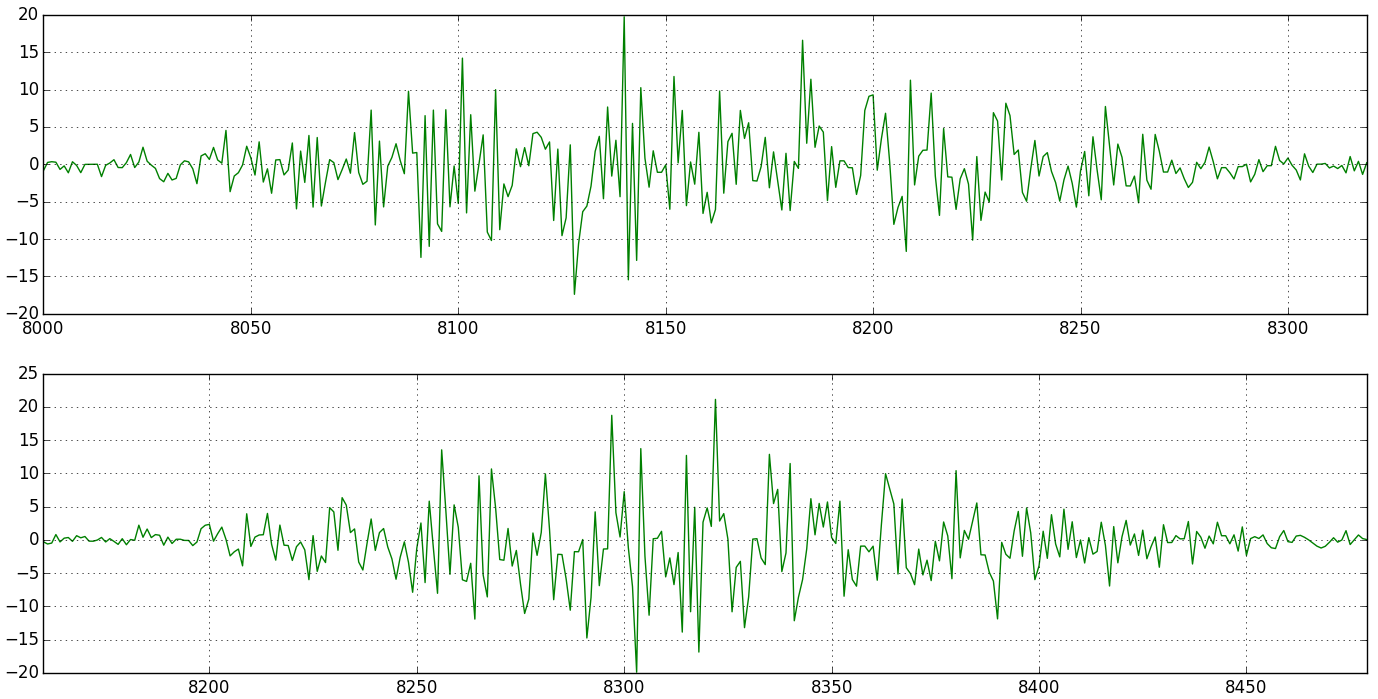
\includegraphics[width=\textwidth]{framing}
    \caption{51º and 52º frames. Notice the initial and final samples of each figure.}
    \label{fig:framing}
\end{figure}

%Fourier Transform

For each frame the Fast Fourier Transform (FFT) is calculated, with number of points greater than the width of the window (usually 512). Finally, the modulus of the FFT is calculated and the power spectrum is obtained. Due to its symmetry, only half of the points are kept.

\begin{figure}[ht]
    \centering
    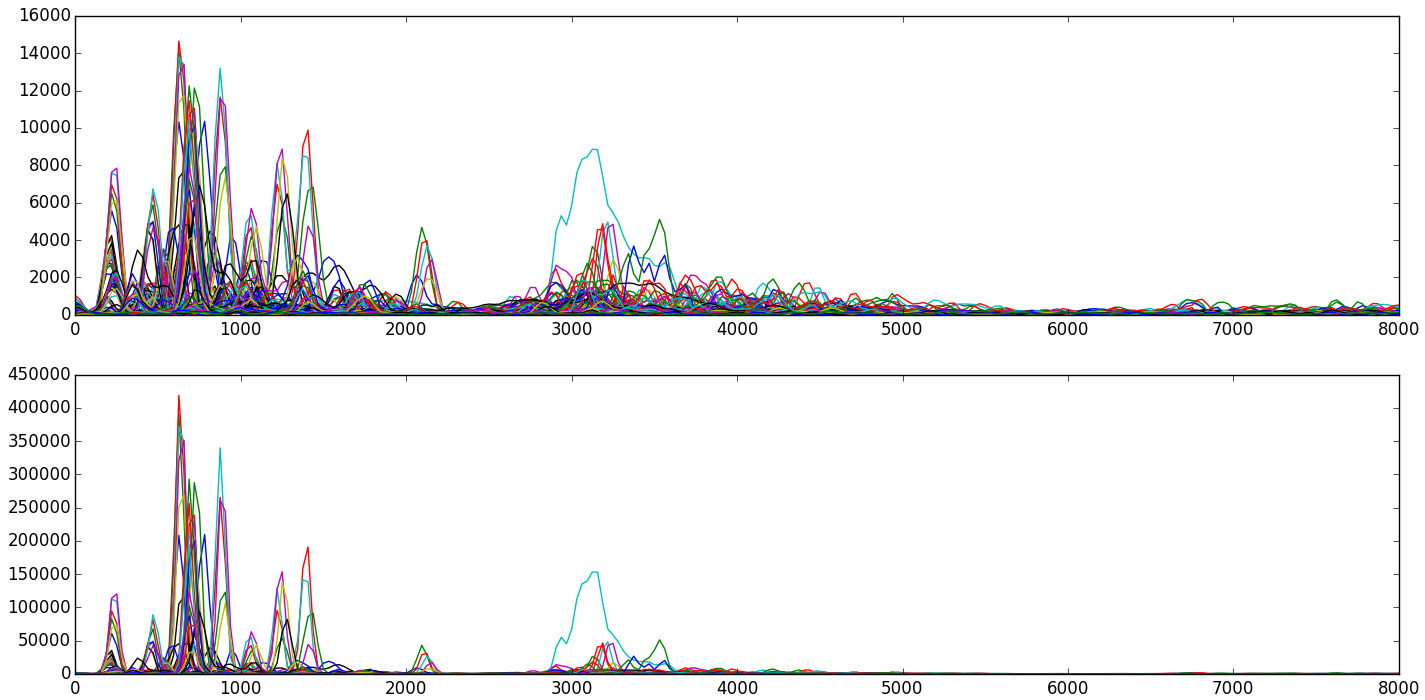
\includegraphics[width=\textwidth]{fft}
    \caption{$|FFT|$ (top) and $|FFT|^2$ (bottom)}
    \label{fig:fft}
\end{figure}

%Filterbank

To get the envelope (and to reduce the size of spectral coefficients), the spectrum is multiplied by a filterbank in the mel scale. As seen in \figureref{filterbank}, the width of the filters enlarge when the frequency increases (these frequencies bands have the same width in mels). This is an approximation of the filtering process executed by the cochlea (see \figureref{cochlea}), and is done this way due to the higher accuracy of human hearing in lower frequencies than in higher ones. The result of the filtering is the energy in each sample of the frame (see \figureref{features_and_featuresdB} (left)).

\begin{figure}[ht]
    \centering
    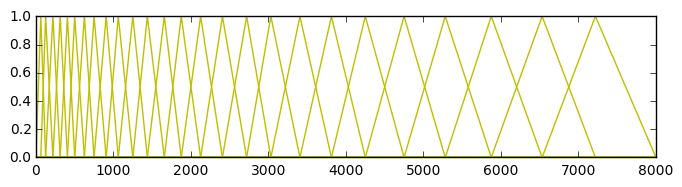
\includegraphics[width=\textwidth]{filterbank}
    \caption{Filter bank with 22 filters.}
    \label{fig:filterbank}
\end{figure}

%Log Conversion

The spectral coefficients are then converted to dB by the application of the function $20\log(\cdot)$ to each sample of each frame, reducing the differences between energy values.

\begin{figure}[ht]
    \centering
    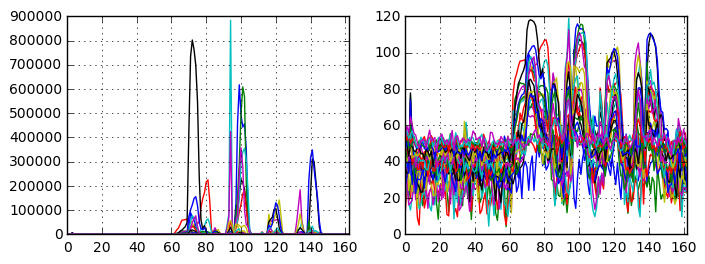
\includegraphics[width=0.9\textwidth]{features_and_featuresdB}
    \caption{Spectral coefficients after the filterbank (left) and after the log conversion (right).}
    \label{fig:features_and_featuresdB}
\end{figure}

%DCT

Until now the features are in the mel scale, but are not yet ``cepstral". The last necessary stage is to apply a Discrete Cosine Transform (DCT) to the spectral coefficients in order to yield the cepstral coefficients:

\begin{equation}
    c_n = \sum_{k=1}^K S_k\cdot\cos\left[n\left(k - \frac{1}{2}\right)\frac{\pi}{K}\right],\qquad n = 1, 2, ..., L,
    \label{eq:dct}
\end{equation}

\noindent where $K$ is the number of spectral coefficients, $S_k$ is a spectral coefficient, and $L$ is the number of cepstral coefficients to calculate ($L \leq K$). The application of a lifter (a cepstral filter) is usual after the computation of the DCT, to smooth the coefficients. After this stage, the MFCCs are extracted.

\begin{figure}[ht]
    \centering
    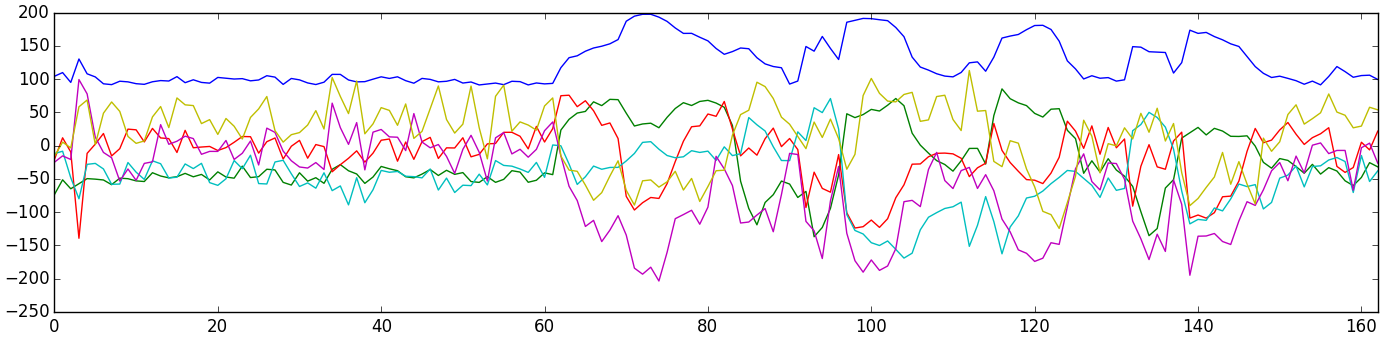
\includegraphics[width=\textwidth]{mfcc}
    \caption{6 MFCCs for each frame over.}
    \label{fig:mfcc}
\end{figure}

%Append Energy

In \figureref{mfcc}, the blue line represents the first feature, and as it is clear, its values over time are much higher than the values of the others. To correct this discrepancy, the feature is changed by the summed energy of each frame, bringing it closer to the others (see \figureref{mfcc_energy_appended}).

\begin{figure}[ht]
    \centering
    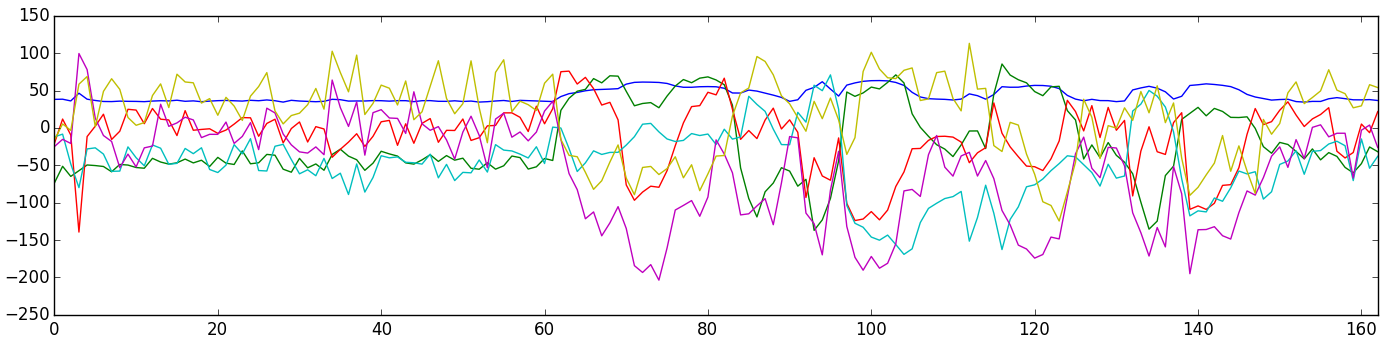
\includegraphics[width=\textwidth]{mfcc_energy_appended}
    \caption{First feature changed by the summed energy of each frame.}
    \label{fig:mfcc_energy_appended}
\end{figure}

%Cepstral Means Subtraction

Even an utterance recorded in a quiet environment still suffers with the side effects of any noise captured during the recording, what may degrade the performance. For speeches recorded in regular places (e.g., a living room or a park), the environment robustness is a need. Cepstral Means Subtraction (CMS),

\begin{equation}
    c_n = c_n - \frac{1}{T} \sum_{t=1}^T c_{n,t},
    \label{eq:cms}
\end{equation}

\noindent reduces the disturbing channel effect before the ASR system be trained, delivering a cleaner signal to the models, \refbib{Westphal}{westphal.1997}.

%Delta Coefficients

In order to improve the speech parameters, the differences in time around each coefficient may be added as new features. In a vector with 6 features per frame, the velocity and acceleration of each coefficient may be added, providing 12 more features to the parametrization, all of them related to the ones previously extracted. These new features are the \textbf{deltas} of the MFCCs, given by

\begin{equation}
    d_t = \frac{\sum_{n=1}^N n(c_{t+n} - c_{t-n})}{2\sum_{n=1}^N n^2}.
    \label{eq:deltas}
\end{equation}

\noindent where $N$ determines how far from the frame $t$ the calculation is taken. \figureref{mfcc_energy_appended_cms_delta_order_2} shows the MFCCs from \figureref{mfcc_energy_appended_cms} improved by the addition of deltas of first and second orders.

\begin{figure}[ht]
    \centering
    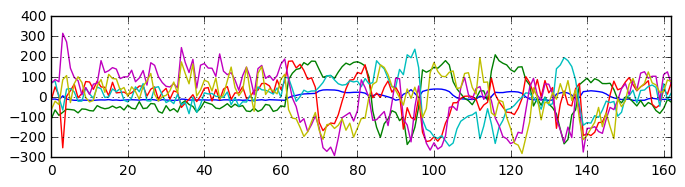
\includegraphics[width=\textwidth]{mfcc_energy_appended_cms}
    \caption{CMS applied to the MFCCs from \figureref{mfcc_energy_appended}.}
    \label{fig:mfcc_energy_appended_cms}
\end{figure}

\begin{figure}[ht]
    \centering
    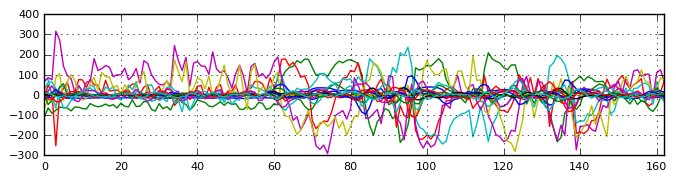
\includegraphics[width=\textwidth]{mfcc_energy_appended_cms_delta_order_2}
    \caption{MFCCs from \figureref{mfcc_energy_appended_cms} with deltas of order 1 and 2 added.}
    \label{fig:mfcc_energy_appended_cms_delta_order_2}
\end{figure}

\equationref{deltas} may be used to calculate deltas of any order, just as the acceleration (second order) is derived from the velocity (first order). However, as seen in \figureref{mfcc_energy_appended_cms_delta_order_2}, each order of delta delivers lower coefficients, providing a more marginal gain with the increase in order.